%We present the experimental results of \sys's performance. We start with describing the hardware environment (Section~\ref{sec:results_hardware}) followed by the software environment (Section~\ref{sec:results_software}) and we concluded by the evaluation results (Section~\ref{sec:results_evaluation}).

We evaluated \sys using a WISP\,5.1~\cite{wisp5,wisp} energy-harvesting
platform build around a MSP430FR5969~\cite{wolverine} MCU with 64\,kB of FRAM.
We used a TI Flash Emulation Tool (FET)~\cite{fet} as a power supply during
experiments with continuous power. For energy measurements, we used
EDB~\cite{edb}. In experiments with wireless power, we powered the WISP using
an RFID reader (Impinj R1000 with firmware version
3.2.4.240~\cite{r1000_data_sheet}) connected to the Liard RFMAX S9028PCRJ
8\,dBic~\cite{atlas2015}. We controlled the RFID reader from a workstation
running Ubuntu 10.4 using \emph{sllurp}~\cite{sllrp_github}. We set the
transmitted power of the RFID reader to 30\,dBm at 915\,MHz center frequency.
For distance-controlled experiments, we affixed the WISP at varying lengths to
hollow paper tubes placed flat on a lying antenna. Timing measurements
were done using the Salea~\cite{saleae} logic analyzer.

For some experiments (noted below) we used an alternative setup where the
MSP-TS430RGZ48C launchpad was used for continuous power experiments and used
internal timer for measuring run time. For harvested energy, we used
WISP\,5.0~\cite{wisp5,wisp} hardware and ThingMagic Astra-EX integrated RFID
reader set at 30\,dBm transmission power at 915\,MHz. We used EDB~\cite{edb}
to measure run time. Applications were cross-compiled using GCC and Clang (both version 3.8.0), allowing us to use LLVM for the \sys compiler. 

\subsection{Benchmarks and Baseline}
\label{sec:results_software}

We compare \sys against state-of-the-art task-based runtime Chain~\cite{chain}.
We do not compare \sys to other, earlier systems, such as DINO~\cite{dino} or
Mementos~\cite{mementos} (cf. Section~\ref{sec:background_consistency}), as
Chain is the only task-based execution model available to which we can compare
\sys. 

We evaluated \sys using benchmarks from the literature~\cite{chain,alpaca} and
several new programs: (i) \textbf{bc}: counts bits in byte pseudo-random string
using several algorithms, and compares results for correctness; (ii)
\textbf{cem}, which emulates an embedded temperature sensing engine and in
which measurements are randomly generated and compressed using LZW with a fixed
entry dictionary and fixed byte block; (iii) \textbf{cuckoo}: which implements
a Bloom-filter-like Cuckoo filter that first hashes a sequence of pseudo-random
numbers, then queries the filter to recover the sequence; (iv) \textbf{rsa}:
which encrypts a fixed string with a stored key; (v) \textbf{ar}: which
performs nearest neighbour classification of randomly generated data modelling a
three-axis accelerometer. This set of benchmarks overlaps with those used
in~\cite{chain,alpaca}. We implemented several new applications: (vi)
\textbf{sort}: selection sort algorithm on a fixed sequence of numbers, and
(vii) \textbf{dft}: discrete Fourier transform. All applications are compared
in columns eight and nine of Table~\ref{table:compiler_result} showing the
number of source lines of code compared to Chain.

%\begin{table}[t]
%	\centering
%	\footnotesize
%	\begin{tabular}{|c|c|c|}
%		\hline
%		Application & SLOC (\sys) & SLOC (Chain~\cite{chain})\\
%		\hline\hline
%		{bc} & 351 & 588 \\ %59\%
%		{cem} & 388 & 721 \\ %53\%
%		{cuckoo} & 483 & 762 \\ %63\%
%		{rsa} & 887 & 1233 \\ %71\%
%		{ar} & 483 & 762 \\ %63\%
%		{dft} & {} & {} \\ %Two resolutions: 4 and 8 Bytes
%		{dd} & {} & {} \\ %Data decompression size: 100 bytes
%		{sort} & {} & {} \\
%		\hline
%	\end{tabular}
%\caption{List of benchmark programs used in \sys evaluation; SLOC: source lines of code.}
%\label{table:benchmark_list}
%\end{table}

\subsection{\sys Evaluation Results}
\label{sec:results_evaluation}

We evaluated \sys to show that it is easy to use and efficient across our
benchmarks. %We evaluate \sys's ease of use by characterizing \sys's automatic task compiler. We evaluate \sys efficiency by comparing its runtime performance to Chain. We characterize \sys by studying how its performance varies due to coalescing and when using automatic task compilation versus manual task compilation.

%\begin{table}[t]
%	\centering
%	\footnotesize
%	\begin{tabular}{|c|c|c|c|c|c|}
%		\hline
%		bc & cem & cuckoo & rsa & ar & sort \\
%		\hline\hline
%		3 & 2 & 6 & 86 & 34 & < 1 \\
%		\hline
%	\end{tabular}
%	\caption{\sys compile time per application (seconds).}
%\label{table:compile_time}
%\end{table}
%
%\subsubsection{Task Coalescing Performance}
%\label{sec:results_coalescing}

%List of figures: 
%\begin{itemize}
%	\item Fig. 1: Viper only/per app/fixed power/(hand/complier)/no coalescing/clang [Resuls are ready by Kiwan]
%	\item Fig. 2: Viper only/per app/per distance (fixed/20/40/60)/(hand/complier)/coalescing [Resuls are ready by Kiwan]
%	\item Fig. 3a: (Viper Coalescing/Chain)/per app/per distance (fixed/20/40/60)/complier/clang [Resuls are ready by Kiwan]
%	\item Fig. 3b: (Viper Coalescing/Chain)/per app/per distance (fixed/20/40/60)/complier/gcc [Resuls are not ready: Kiwan needs to make them]
%	\item Fig. 4: exactly as Fig 12 in the paper (4 apps only)
%	\item Fig. 5: average virtual task size/gcc/fixed distance/per app 
%\end{itemize}

\subsubsection{\sys Runtime Performance}
\label{sec:result_coalescing}

\begin{figure}
	\centering
	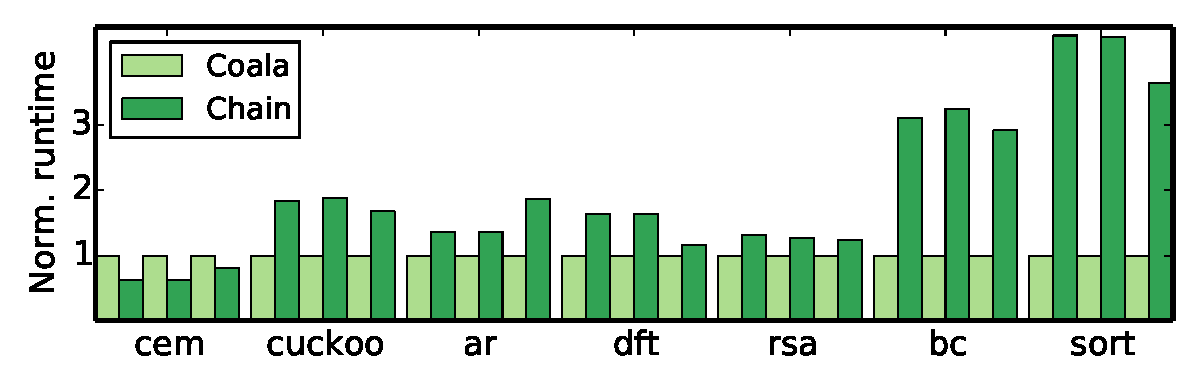
\includegraphics[width=\columnwidth]{figures/coala_chain_clang}
	\caption{\textbf{Performance of \sys applications (divided manually into tasks) at multiple WISP to RFID reader antenna distances}: fixed power (0\,m to the antenna) and \{0.2, 0.4\}\,m (left, center and right-most bar per application, respectively), compared against Chain (results are normalized).}
	\label{fig:runtime}
\end{figure}

\textbf{\sys versus Task-based Model.} We evaluate \sys's run time performance and compare \sys to the run time performance of Chain. Results are given in Figure~\ref{fig:runtime}. For each application we measured its execution time on continuous power, i.e. 0\,m RFID antenna/WISP distance (the first two bars of each group) and on intermittent power at 20\,cm and 40\,cm from the RFID antenna (the second two and third two bars of each group, respectively). The data show the average execution time of each application run repeatedly for 20 seconds, with runtimes normalized to \sys's average. The results show that \sys provides a performance benefit compared to Chain for most applications. The performance benefit is greatest for applications that have small tasks (bc, sort, cuckoo) at all distances on intermittent power and with fixed power. In applications that have larger tasks (e.g. dft) or access more different memory pages, \sys incurs overhead from memory virtualization that cause its performance to be comparable to (or in the \emph{single} cem case, worse than) Chain. 

\textbf{Coalescing Strategies.} We evaluated the impact that \sys's dynamic task coalescing had on run time performance.  Figure~\ref{fig:coalescing} shows the run time performance of \sys's coalescing, compared to \sys running without coalescing enabled with data normalized to the run time performance of \sys with coalescing.  We show data from experiments with continuous power (the first two bars in each bar
group), and with intermittent power, with the WISP at 20\,cm and 40\,cm from the
RFID reader (the second and third groups of two bars in each group). The data illustrate that coalescing improves \sys's performance by eliminating the overhead of committing after each task.  The performance benefit varies, providing up to 4.5x performance improvement (for cuckoo filtering, at 40cm). The cuckoo application (like other top-performers, bc and sort) has small tasks that \sys can easily coalesce to eliminate many commits. In contrast, for some applications, e.g. cem, coalescing does not improve performance. The reason for cem's poor performance is that cem uses a large LZW dictionary structure that spans multiple pages, but has very little {\em locality}. The absence of locality means that coalesced tasks do not access the same pages, and as a result, do not amortize commit overhead. The lack of locality causes performance to regress to be similar to the non-coalescing case. 

%Uniformly distributed random pattern of power interrupts with an average on and off time of 15\,ms and 10\,ms respectively.

\begin{figure}
	\centering
	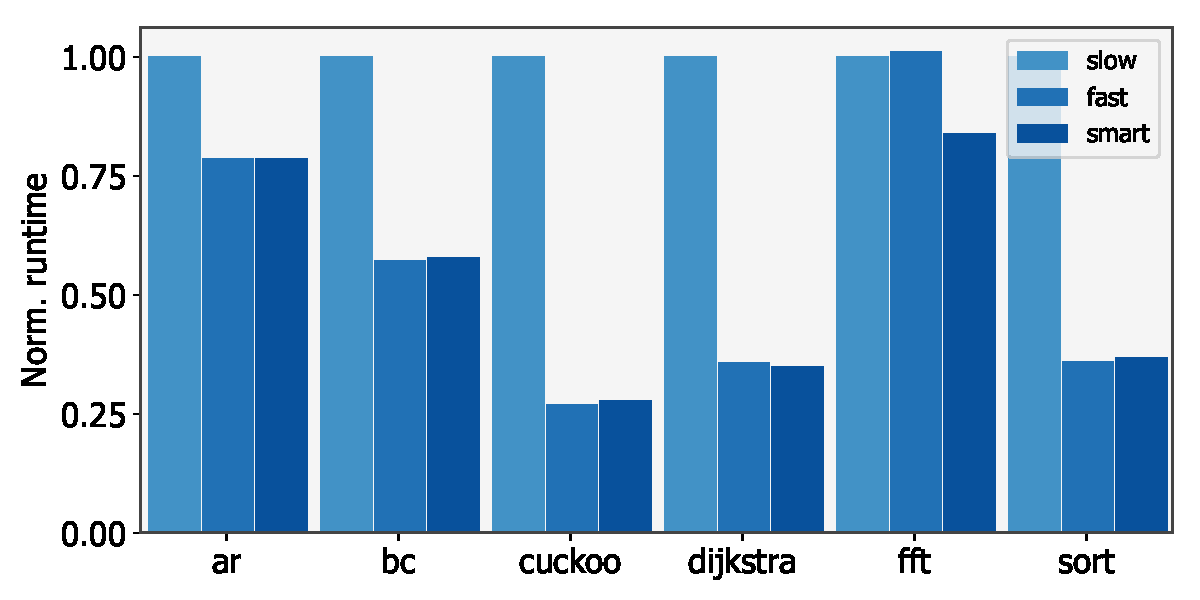
\includegraphics[width=\columnwidth]{figures/coalStrategies}
	\caption{\textbf{\sys coalescing strategies (`WHD' and `HD') performance per application on intermittent power compared to \sys without coalescing (`NO').} Coalescing provides benefit for all applications, while we observe little difference between `WHD' and `HD'.}
	\label{fig:coalescing}
\end{figure}

%\begin{table}
%	\centering
%	\footnotesize
%	\begin{tabular}{|r|c|c|c|}
%		\hline
%		{} & bc & dft & cem \\
%		\hline\hline
%		Avg. no. coalesced tasks & 56 & 3 & 26 \\
%		Avg. task size (MCU cycles) & 657 & 9680 & 722 \\
%		\hline
%	\end{tabular}
%\caption{Average \sys virtual task size (at 60\,cm WISP to RFID antenna distance) per manually task split application.}
%\label{tab:aveVirtuTaskSize}
%\end{table}

%\begin{figure}
%	\centering
%	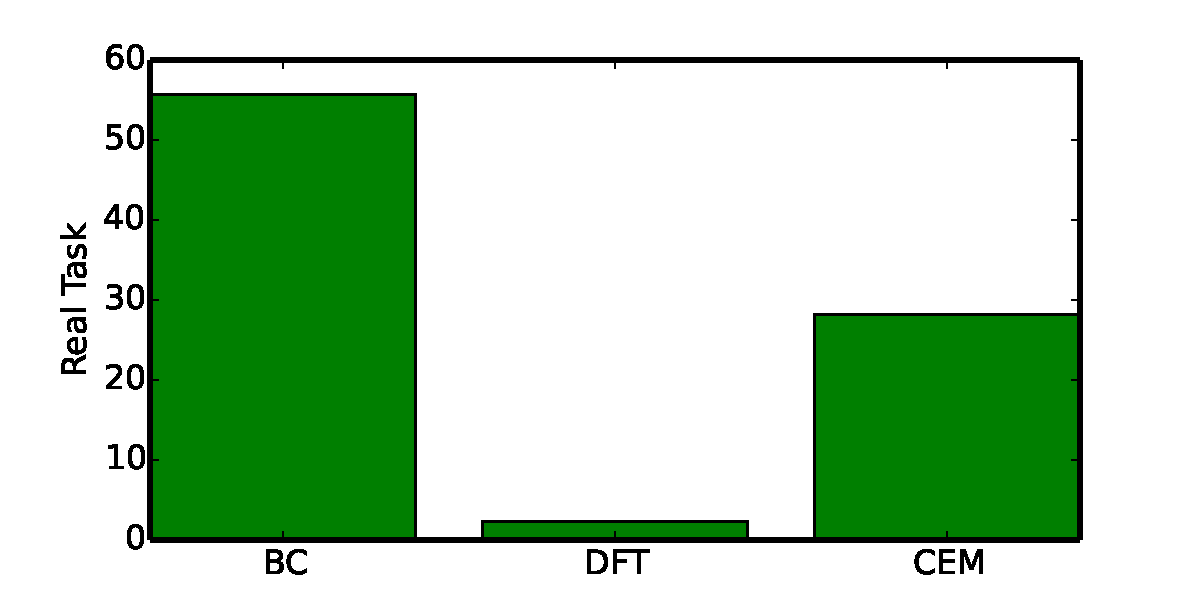
\includegraphics[width=\columnwidth]{figures/averageVirtualTaskSize}
%	\caption{Average \sys virtual task size at fixed power per application. Top (green): number of coalesced tasks; bottom (red): average size of real task.}
%	\label{fig:aveVirtuTaskSize}
%\end{figure}

%Then, we need to know how many tasks \sys can coalesce within a given execution scenario. We ran a subset of applications (split by tasks manually) with continuous power supply and measured the size of tasks for each application and the amount of tasks coalesced. Result is given in Table~\ref{tab:aveVirtuTaskSize}. We see clearly that \sys manages to coalesce more tasks as individual tasks are small. As the size of individual task increases, e.g., as in the case of dft application, the number of coalesced tasks is also small. This result clearly shows that for the benefit of coalescing and for code portability, initial code should be split by \emph{as small tasks as possible}. This will help \sys to find the best possible virtual task size to minimise its runtime.

\subsubsection{\sys Paging Performance}
\label{sec:results_memory_management}

We evaluated the effect that paging with different page sizes has on \sys's performance and we show data in Figure~\ref{fig:page_size}; The top plot shows the run time performance normalized to the best per-application performance, using pages of different sizes in \sys, indicated with the labels at each bar; the bottom plot shows the number of page faults for the same set of executions normalized to the maximum of each set. We measured performance as MCU clock cycles using values read out by TI's CCS IDE. The results show a clear ``bathtub curve'' in the performance of each application, as the number of page faults varies. The data show that across application there is a page size that minimizes \emph{both} execution time. We observe that the page size is not the same for each application, although 64 byte pages perform well for all applications. The increased rate of page faults is responsible for the overhead with small page sizes; smaller pages require accessing more different pages, leading to higher paging costs. With larger page sizes, the overhead is higher than with moderate pages, too. The explanation for these higher overheads is that large pages have a higher commit cost. Even if an application accesses few memory locations, \sys pages data at full page size, degrading performance by sometimes paging in and out unnecessary data. The data reveal a reasonable default page size of 64 bytes and when developing an application, a developer should consider varying the page size to moderate poor performance.

\begin{figure}
	\centering
	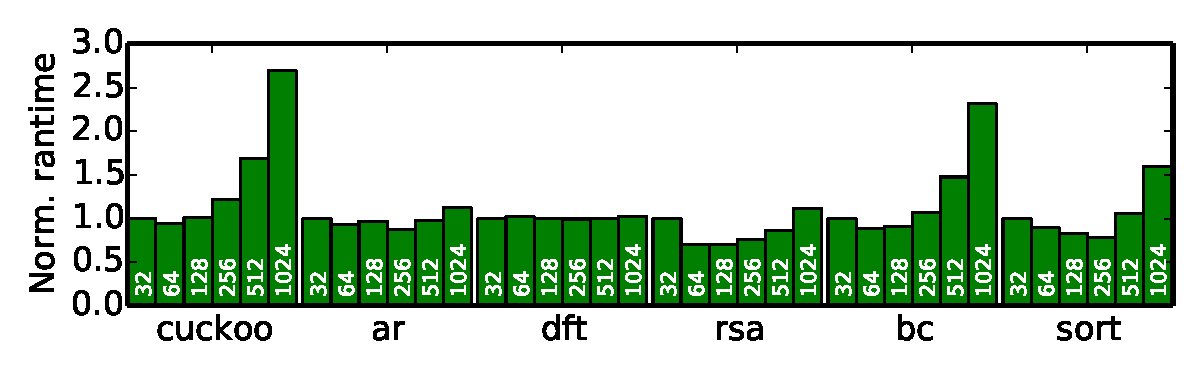
\includegraphics[width=\columnwidth]{figures/ramPagsSizes}
	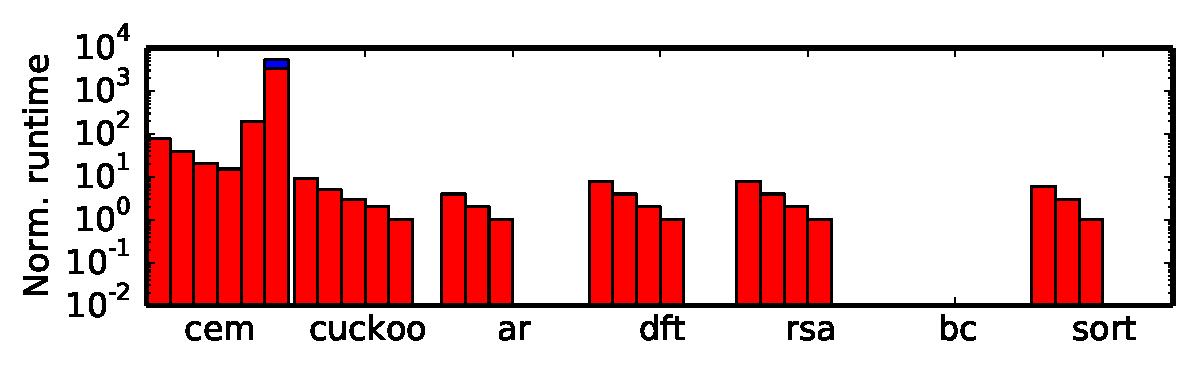
\includegraphics[width=\columnwidth]{figures/pagefault}
	\caption{\textbf{\sys normalized runtime for various page sizes, \{32, 64, $\ldots$,1024\}\,bytes, per application (top) and respective page faults (bottom)}; X: no page faults.}
	\label{fig:page_size}
\end{figure}

\subsubsection{\sys's Compiler}
\label{sec:result_compiler_time}

\begin{table}[t]
	\centering
	\footnotesize
	\renewcommand{\tabcolsep}{1pt}
	\begin{tabular}{|l|cc|cc|cc|cc|c|}
		\hline
		{} & \multicolumn{2}{c|}{{\bf Prot. bytes}} & \multicolumn{2}{c|}{{\bf \# Tasks}} & \multicolumn{2}{c|}{{\bf \# Prot. acc.}} & \multicolumn{2}{c|}{\bf SLOC} & {\bf Comp.} \\
		App & Man. & Comp. & Man. & Comp. & Man. & Comp. & \multicolumn{1}{l}{\sys} & \multicolumn{1}{r|}{Chain~\cite{chain}} & {\bf time} \\
		\hline\hline
		bc & 22 & 22 & 10 & 15 & 81 & 93 & 351 &588 & 3\\
		cem & 3492 & 3242 & 12 & 9 & 92 & 123 & 388 &721 & 2\\
		cuckoo & 282 & 288 & 15 & 6 & 90 & 76 & 483 &762 & 6\\
		rsa & 332 & 250 & 20 & 27 & 130 & 296 & 887 &1233 & 86\\
		ar & 166 & 218 & 11 & 6 & 112 & 333 & 483 &762 & 34\\
		sort & 104 & 104 & 4 & 2 & 70 & 23 & 180 & 287 & $<$1\\
		dft$^\dagger$ & --- & --- & --- & --- & --- & --- & 222 & 293 & ---\\
		%dd &  &  &  &  &  &  &  & 287 &  \\
		\hline
	\end{tabular}
	\caption{\textbf{Comparison between \sys and Chain source code line number (SLOC column) and comparison between compiler-generated \sys code (Comp.) and hand-written \sys code (Man.) (other columns)}; $^\dagger$dft does not compile with Clang}\label{table:compiler_result}
\end{table}

\textbf{\sys Compiler Generated Code Characterization.} The behaviour and the efficiency metrics of the \sys compiler are given in Table~\ref{table:compiler_result}. 
%
%for each application, for manually written (Man.) and automatically compiled (Comp.) benchmarks the difference in the number of bytes of protected data (columns 2 and 3), the number of tasks (columns 4 and 5), the number of \sys protected data API access calls (columns 6 and 7), the lines of code in each application for \sys and Chain (columns 8 and 9), and compilation time using \sys's compiler (column 10).
%
On average, compiler-generated code introduces about 0.3\% more bytes of protected data, suggesting that liveness analysis captures natural boundaries in the use of variables also caught by a manual implementation. Compiler-generated code generates about 16\% fewer tasks for applications, on average. The results indicate that the \sys compiler selects task boundaries differently than a programmer would manually, favoring fewer, larger tasks. The \sys compiler inserts protected data access operations conservatively when a variable {\em may} alias a protected variables, due to the limitations of pointer aliasing. Consequently, the \sys compiler introduces 48\% more protected data accesses than programmer-written code. The run time results in Section~\ref{sec:result_compiler_time} show that the increase in protected data
accesses sometimes degrades performance. Overall, the data show that the compiler automatically generates tasks similarly to manually written tasks. Doing so, \sys's compiler reaps the static task benefits of \sys, but simplifies programming by sparing the programmer the job of task decomposition.

\textbf{Compile Time.} We measured compile time for \sys's compiler's automatic task generation for each application\footnote{We could not compile the dft application since LLVM inserts mathematical built-in functions (i.e. \texttt{\_\_muldf3}, \texttt{\_\_floatsidf}, \texttt{\_\_adddf3}) whose implementation were not provided by the LLVM MSP430 back-end.}. We compiled the applications on a 4-core virtual machine with 1\,GB of memory running Arch Linux on an Intel Core i5-6200U at 2.30\,GHz. We collected results using the Linux system time collected in seconds. Most of the compile time was spent computing pointer alias analysis, while calculating the possible live ranges of variables. Applications such as rsa that have a larger code size and manipulate more variables have a longer compilation time, due to a larger search space for pointer aliasing. Nonetheless, the compile time is orders of magnitude shorter than manually defining tasks, which requires hours of programmer time. %The characterization of \sys's compiler suggests that the \sys compiler enables simpler task-based intermittent programming for \sys.

\textbf{Run Time of \sys Compiler Code.} In addition to the characterization of the \sys compiler in Table~\ref{table:compiler_result}, we experimentally assessed the performance of the \sys compiler, compared to the performance of the manually written benchmarks, as written in prior work~\cite{alpaca,chain}. Figure~\ref{fig:comp_user} compares the performance of manually written benchmark code to the performance of code automatically compiled using \sys. The figure shows run time for both cases, normalized to the run time of the manually written program, running on continuous power. The data show that in all cases except for ar and rsa, the run time performance of compiled code generated by the \sys compiler has comparable performance to manually written code. With comparable performance in most cases, the data suggest that the \sys compiler not only makes programming simpler, but does so, in most cases, without a high run time overhead. In the cases of both ar and rsa, the code manipulates a large amount of data that is stored in an array and passed into functions by reference. We expect that the data being manipulated by reference is leading to a large amount of may-alias references in the compiler's analysis, which leads to a larger number of accesses to protected data in the automatically compiled code, compared to the manually written code.

\begin{figure}
	\centering
	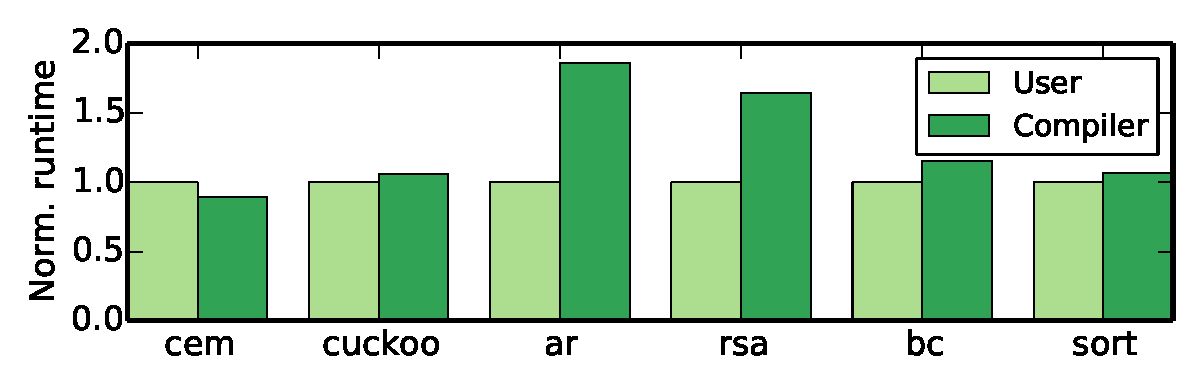
\includegraphics[width=\columnwidth]{figures/comp_user}
	\caption{\textbf{\sys compiler code overhead measured in terms of execution time per application} (dft excluded as it was not compiled by \sys compiler, see Table~\ref{table:compiler_result}); WISP was powered continuously.}
	\label{fig:comp_user}
\end{figure}

%\subsubsection{Case Study}
%\label{sec:case_study}

%The final experiment assessing usefulness of \sys's use in real application. For this we have a implemented an battery-less wirelessly-powered sound detector as an example. To the best of our knowledge, this is the first case study that demonstrates a intermittently-powered system supplied by harvested energy at runtime, which continuously interacts with real-life signals. 

%The application aims at detecting a specific tone in the audio signal (in the implementation: 1\,kHz) based on on-the-fly audio measurement. For this we have connected an analog MEMS microphone~\cite{microphone} output to AUX3 port of WISP\,5.1 (while the microphone was powered directly by WISP, which was then wirelessly power-supplied by the RFID reader). Audio signal is sampled by the microcontroller's ADC and passed to the FFT function (internal function of the TI's Digital Signal Processing library~\cite{ti_dsp}) to find a tone above a predefined threshold. The output of the detection is signalled by the WISP on-board LED. The video of demonstrating the working system is available via \url{https://link_to_a_video}.

%Expected results:
%\begin{itemize}
%	\item Compare execution time: \sys against Chain for X\,s long audio signal detection at two antenna distances
%	\item Make a video of the demonstration 
%\end{itemize}
 
%\todo{Check if we really need this application}{Brandon}
%\todo{Provide results and text to this section---if time allows (this result is not critical)}{Amjad/Przemek}
